% Created 2017-11-16 Thu 00:31
\documentclass{article}
\usepackage[utf8]{inputenc}
\usepackage[T1]{fontenc}
\usepackage{fixltx2e}
\usepackage{graphicx}
\usepackage{longtable}
\usepackage{float}
\usepackage{wrapfig}
\usepackage{rotating}
\usepackage[normalem]{ulem}
\usepackage{amsmath}
\usepackage{textcomp}
\usepackage{marvosym}
\usepackage{wasysym}
\usepackage{amssymb}
\usepackage{hyperref}
\tolerance=1000
\usepackage{tabularx,graphicx,ragged2e,booktabs,caption,float}
\usepackage[margin=0.8in]{geometry}
\usepackage{amsmath}
\usepackage{gensymb}
\usepackage{authblk}
\setlength{\parskip}{0.2cm}
\setlength{\parindent}{0.85cm}
\author{Tiankai Xiong}
\date{\today}
\title{PC5215, Lab4}
\hypersetup{
  pdfkeywords={},
  pdfsubject={},
  pdfcreator={Emacs 25.3.1 (Org mode 8.2.10)}}
\begin{document}

\maketitle

\section{Part A}
\label{sec-1}

The problem of a one dimensional scattering over a potential barrier
has been well studied and the solutions are readily available. The
derivation is tedious and time-consuming which will not be presented
here. The solutions for transmission coefficient for a square
barrier with

$$V_1(x < 0) = 0, \quad V_1(0\leq x < a) = V_0, \quad V_1(x \geq a) = 0$$

is

$$T = |c|^2 = [1+ \frac{V_0^2 sinh^2(k_1 a)}{4E(V_0-E)}]^{-1}$$

for $E < V_0$, and

$$T = |c|^2 = [1+ \frac{V_0^2 sin^2(k_2 a)}{4E(E-V_0)}]^{-1}$$

for $E> V_0$ where $k_1 = \sqrt{2m(V_0-E)/\hbar^2}$, $k_2 = \sqrt{2m(E-V_0)/\hbar^2}$

The plot for transmission coefficient T for $E \in [0, 2eV]$ with
the square potential $V_0 = 1 eV$ is presented in Figure
\ref{fig:analytic}. It will serve as a reference for the following parts.

\begin{figure}[h]
  \centering
  \includegraphics[width = 0.7\textwidth]{Analytic.pdf}
  \caption{Transmission coefficient for square potential $V_0 = 1 eV$ with $E \in [0, 2 eV]$}
  \label{fig:analytic}
\end{figure}

\section{Part B}
\label{sec-2}

\subsection{Theoretical approach}
\label{sec-2-1}
To study the same problem in a computational manner, we define an
1D wave packet concentrated at $(x_0, p_0)$

$$\Psi(x) \propto exp(-\frac{1}{2 \sigma^2}(x-x_0)^2 + \frac{i}{\hbar}p_0(x-x_0))$$

which propagates in the positive x direction.

The time evolution of the wave packet can be described as such

$$\Psi(t+\Delta t) = e^{-\frac{i}{\hbar} H \Delta t}$$

where the Hamiltonian is an operator

$$H = - \frac{\hbar^2}{2m} \frac{\partial^2}{\partial x^2} + V(x)$$

The two parts, represented at $A$ and $B$ respectively, do not
commute. However, Trotter-Suzuki formula

$$e^{A+B} \approx e^A e^B$$

allows us to evaluate the two parts separately. The partial
differentiation is the value of momentum in p space which could be
obtained via Fourier transformation.

The work flow for an evolution by $\Delta t$ is as follows:

$$(1)\quad \Psi(x, t) \to e^{-\frac{i}{\hbar}V(x) \Delta t}\Psi(x,t) = \Psi_{1/2}(x, t + \Delta t)$$
$$(2) \quad \Psi_{1/2}(x, t+\Delta t) \to \Psi_{1/2}(p, t+ \Delta t)$$
$$(3) \quad \Psi_{1/2}(p, t+\Delta t) \to e^{-\frac{i}{\hbar} \frac{p^2}{2m} \Delta t}\Psi_{1/2}(p, t + \Delta t) = \Psi(p, t + \Delta t)$$
$$(4) \quad \Psi(p, t+\Delta t) \to \Psi(x, t+\Delta t)$$

where the conversion between $\Psi(x, t)$ and $\Psi(p, t)$ is done via Fast Fourier Transform(FFT).


\subsection{Implementation}
\label{sec-2-2}

The 1D space is indexed by discrete coordinates $x_i \in \{x_1
   .. x_N\}$. We shift the coordinate such that $x_{N/2} = 0$ which
locates the potential barrier at the center of the space. When
transformed to $p$ space, it ranges from $p = 0$ to $p =
   \frac{N}{2} \Delta p$, then from $p = -\frac{N}{2}\Delta p$ to
$-\Delta p$. $\Delta p$ is determined by the relation between $\Delta x$ and $\Delta p$

$$\frac{\Delta x \Delta p}{\hbar} = \frac{2\pi}{N}$$

We also need to define the spread of the wave packet which is
determined by the standard deviation $\sigma$. In our approach,
$\sigma = a$ is taken so that the original wave packet spans around
the same fraction in each of their spaces. The center of the wave
packet is at $x_0 = -5 \sigma$ so that it is essentially on the
left of the potential barrier in the initial state. The width of
the potential barrier, a, is chosen so that

$$\frac{\hbar^2}{2m a^2} = \frac{1}{100}eV$$

Without having to use any standard unit, we just define $V_0 = 1
   eV$, $\hbar = 1$, $m = 1$ so that $a = 5\sqrt{2}$
and the units agree with each other.

We need to let the wave packet evolve so that in the case where
there is no potential barrier, it is entirely on the right hand
side of the non-existent barrier. This is ensured by having $t \times p_0 =
   20a$ where $p_0$ assembles the group velocity of the wave packet.

The last step is to calculate transmission coefficient. This is
done by Monte Carlo method. We pick random sites from the x space
and only choose to evaluate it should it is has higher probability
density than the previous point, or the ratio of the probability
density at two points surpasses a random variable between 0 and 1.
At the end, we calculate the percentage of those that fall on the
right hand side of the potential barrier which would be the value
of transmission coefficient. 30 samples are taken for each
iteration to conduct statistical analysis.

\section{Part C}
\label{sec-3}

This part is essentially the same as part B except that we need to
define the potential barrier in a inverted parabola fashion.

\section{Results}
\label{sec-4}

Both potentials give a similar T-E curve as compared to the
analytical solution (Figure \ref{fig:T-E}). The arch shape or
inverted parabola potential barrier produces a curve that has a
higher transmission coefficient as compared to the flat block case.
This is due to the fact that while both potential barriers are equal
in height, the arch shaped is effectively "thinner" in width. The
wave packet thus have higher probability to propagate to the right
of if by tunneling. Although the curves look similar to the
analytical solution, they fail to predict the drop in transmission
coefficient between $E = 1$ and $E = 2$.

\begin{figure}[H]
  \centering
  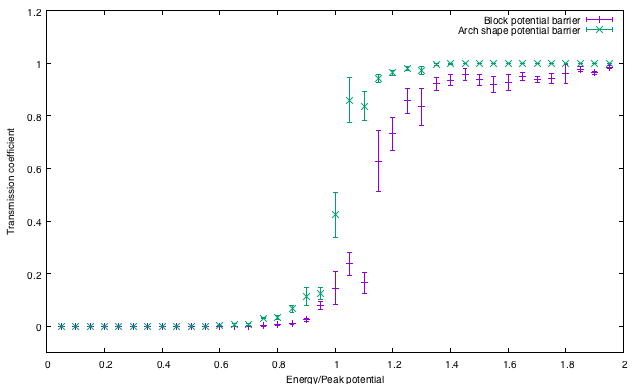
\includegraphics[width=0.9\textwidth]{Transmission_coefficient.png}
  \caption{Transmission coefficient at different energies}
  \label{fig:T-E}
\end{figure}

To visualize the different cases, we have drawn probability
density graph for both cases at four representative energies.(Figure
\ref{fig:05}, \ref{fig:10}, \ref{fig:15}, \ref{fig:20}) At $E = 0.5
  V_0$, the wave packet cannot bypass the barrier and is "bounced
back". At $E = V_0$, about half of the wave packet are able to
propagate to the other side while the rest returned to the left
again. As the energy increases, a larger percentage of the wave
packet propagates to the right. It is also interesting to note that
the original wave packet is more concentrate. It spreads out while
propagating.

\begin{figure}[H]
  \centering
  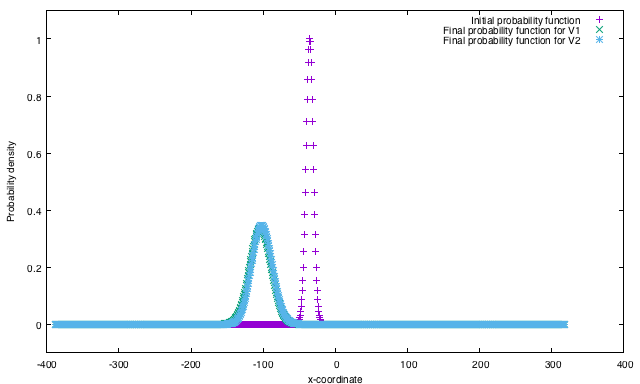
\includegraphics[width=0.9\textwidth]{case05.png}
  \caption{Probability density of wave packet for block potential barrier $V_1$ and arch shape potential barrier $V_2$ at E = 0.5$V_0$}
  \label{fig:05}
\end{figure}

\begin{figure}[H]
  \centering
  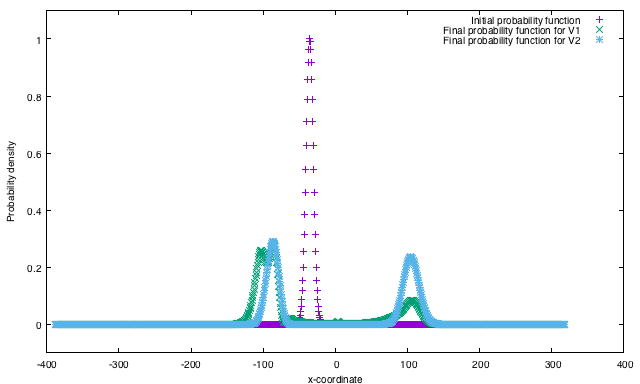
\includegraphics[width=0.9\textwidth]{case10.png}
  \caption{Probability density of wave packet for block potential barrier $V_1$ and arch shape potential barrier $V_2$ at E = 1.0$V_0$}
  \label{fig:10}
\end{figure}

\begin{figure}[H]
  \centering
  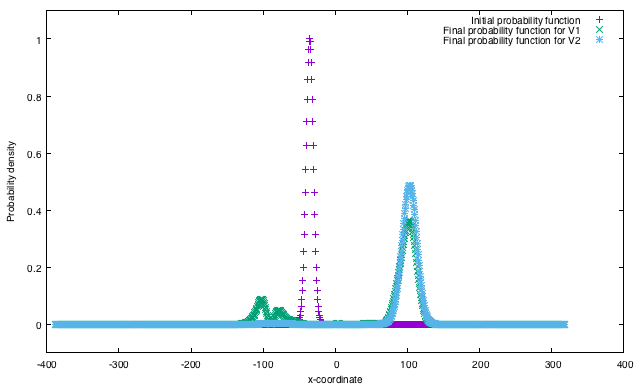
\includegraphics[width=0.9\textwidth]{case15.png}
  \caption{Probability density of wave packet for block potential barrier $V_1$ and arch shape potential barrier $V_2$ at E = 1.5$V_0$}
  \label{fig:15}
\end{figure}

\begin{figure}[H]
  \centering
  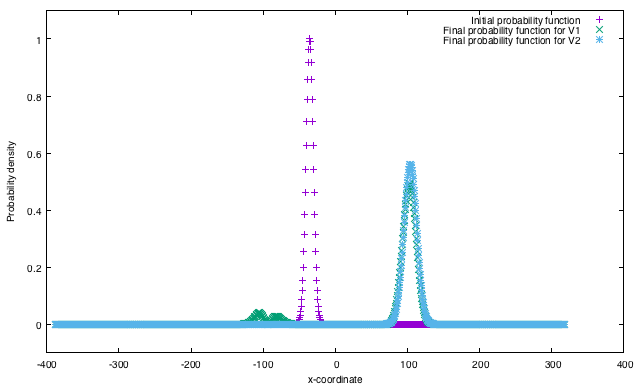
\includegraphics[width=0.9\textwidth]{case20.png}
  \caption{Probability density of wave packet for block potential barrier $V_1$ and arch shape potential barrier $V_2$ at E = 2.0$V_0$}
  \label{fig:20}
\end{figure}

\section{SRC}
\label{sec-5}

\hline
\begin{verbatim}
#include <stdio.h>
#include <stdlib.h>
#include <math.h>

#define SWAP(a, b) tempr = (a); (a) = (b); (b) = tempr

void fouri(double data[], unsigned long nn, int isign){
  /* Replaces data[1..2*nn] by its descrete Fourier transform, if
     isign is input as 1; or replaces data[1..2*nn] by nn times its
     inverse discrete Fourier transform, if isign is input as -1.
     data is a complex array of length nn or, equivalently, a real
     array of length 2*nn, nn MUST be an integer power of 2(this is not
     checked for)*/

  unsigned long n, mmax, m, j, istep, i;
  double wtemp, wr, wpr, wpi, wi, theta;
  double tempr, tempi;

  n = nn <<1;                    /* n = nn * 2 */
  j = 1;
  for(i = 1; i<n; i+=2){        /* This is the bit-reversal section of
                                   the routine */
    if(j > i){
      SWAP(data[j], data[i]);
      SWAP(data[j+1], data[i+1]);
    }
    m=nn;
    while(m >= 2 && j > m){
      j -= m;
      m >>= 1;                  /* m /= 2; */
    }
    j += m;

  }
  /* Here begins the Danielson-Lanczos section of the routine. */
  mmax = 2;
  while(n > mmax){              /* Outer loop executed log_2 */
    istep = mmax <<1;
    theta = isign * (6.28318530717959/mmax); /* Initialize the
                                                trigonometry */
    wtemp = sin(0.5*theta);
    wpr = -2.0 * wtemp*wtemp;
    wpi = sin(theta);
    wr = 1.0;
    wi = 0.0;
    for(m = 1; m< mmax; m+=2){
      for (i = m; i<=n; i+=istep){
        j = i+mmax;
        tempr = wr*data[j] - wi*data[j+1];
        tempi = wr*data[j+1] + wi*data[j];
        data[j] = data[i] - tempr;
        data[j+1] = data[i+1]- tempi;
        data[i] += tempr;
        data[i+1] += tempi;
      }
      wr = (wtemp = wr)*wpr-wi*wpi+wr;
      wi=wi*wpr+ wtemp * wpi + wi;
    }
    mmax = istep;
  }
};

/* Used to calculate the x position */
double x_pos(int N, int j, double x0, double dx){
  if(j<=N){
    return (j-N/2)*dx+x0;       /* The coordinates cover from -N/2*dx
                                   to N/2*dx with a shift by x0 so
                                   that the wavelet in initiated on
                                   the left of the potential
                                   barrier */
  }else{
    printf("Error! j must not exceed N!\n"); /* Just in case */
    return 0;
  }
};

/* Used to calculate the p position */
double p_pos(int N, int j, double dp){
  /* p2 = dp */
  /* p(N/2+1) = N/2*dp*/
  /* pN = -dp */
  double p;
  if(j<=N/2){
    p = (j-1)*dp;         /* ? */
  }else{
    p = (j-N-1)*dp;
  }
  return p;

};

/* To calculate initial values at each x */
void phi_init(double phi_x[], int N, double x0, double dx, double p0, double sigma){
  double part1 = 0;
  double part2 = 0;
  for (int j = 1; j <= N; j++){
    part1 = -1/(2*pow(sigma, 2)) * pow((x_pos(N, j, x0, dx) - x0), 2);
    part2 = p0*(x_pos(N, j, x0, dx)- x0);
    phi_x[2*j-1] = exp(part1)*cos(part2);
    phi_x[2*j] = exp(part1)*sin(part2);
  }
};


/* The definition for a flat block potential */
double V1(double x, double a){
  if(x < 0.0){
    return 0;
  }else if(x < a){
    return 1.0;
  }else{
    return 0.0;
  }

};

/* The definition for a inverse parabolar potential */
double V2(double x, double a){
  if(x < 0.0){
    return 0;
  }else if(x < a){
    return 4/pow(a,2)*(a-x)*x;
  }else{
    return 0.0;
  }

};


void phi_evolve(double phi[], int N, double a, double dt, double v0,
                double dv, char c, int potential){
  double real = 0;
  double imag = 0;
  for(int j = 1; j<= N; j++){
    if(c == 'x'){
      if(potential == 1){
        real = phi[j*2-1] * cos(-V1(x_pos(N, j, v0, dv), a) * dt)
          - phi[j*2]   * sin(-V1(x_pos(N, j, v0, dv), a) * dt);
        imag = phi[j*2]   * cos(-V1(x_pos(N, j, v0, dv), a) * dt)
          + phi[j*2-1] * sin(-V1(x_pos(N, j, v0, dv), a) * dt);
        phi[j*2-1] = real;
        phi[j*2] = imag;
      }else if (potential == 2){
        real = phi[j*2-1] * cos(-V2(x_pos(N, j, v0, dv), a) * dt)
          - phi[j*2]   * sin(-V2(x_pos(N, j, v0, dv), a) * dt);
        imag = phi[j*2]   * cos(-V2(x_pos(N, j, v0, dv), a) * dt)
          + phi[j*2-1] * sin(-V2(x_pos(N, j, v0, dv), a) * dt);
        phi[j*2-1] = real;
        phi[j*2] = imag;
      }

    }else if(c == 'p'){
      real = phi[j*2-1] * cos(-pow(p_pos(N, j, dv), 2)/2 * dt)
        - phi[j*2]   * sin(-pow(p_pos(N, j, dv), 2)/2 * dt);
      imag = phi[j*2]   * cos(-pow(p_pos(N, j, dv), 2)/2 * dt)
        + phi[j*2-1] * sin(-pow(p_pos(N, j, dv), 2)/2 * dt);
      phi[j*2-1] = real;
      phi[j*2] = imag;
    }else{
      printf("Error! Must specify either x or p.\n");
      break;
    }
  }
};

/* Used to plot the density function of the wave function to visualize
   the propogation of wavelet */
void export_DF(double phi_x[], int N, double x0, double dx, FILE *file, char type){
  for(int i = 1; i<= N; i++){
    double x;
    if(type =='x'){
      x = x_pos(N, i, x0, dx);
    }else if(type =='p'){
      x = p_pos(N, i, dx);
    }else{
      x = 0;
    }
    double DF = pow(phi_x[2*i -1],2) + pow(phi_x[2*i], 2);
    fprintf(file, "%f    %f\n", x, DF);
  }

};

/* To normalize the wavefunction so that it does not become N*phi
   after a forward and backward FT */
void normalize(double phi[], int N){
  for(int j = 1; j <= 2*N; j++){
    phi[j] /= sqrt((double)N);
  }
};

double mean(double list[], int N){
  double mean = 0;
  for(int i = 0; i< N; i++){
    mean += list[i];
  }
  return mean/(double)N;
};

double standarderr(double phi[], int N){
  double mu =  mean(phi, N);
  double dummy = 0.0;
  for(int i = 0; i<N; i++){
    dummy += pow(phi[i]-mu, 2);
  }
  dummy /= N-1;
  return sqrt(dummy);
};

int main(){
  double a = 5*sqrt(2.0);       /* a is chosen such that hbar^2/(2ma^2) = 1/100 eV */
  double E;                 /* Energy starts from 0 */
  double p0;        /* momentum follows E = p^2/(2m) */
  int N = pow(2,10);             /* N must be a power of 2 */
  double dx = 100*a/N;             /* arbitrary dx */
  double dp = 2.0*M_PI/(double)(N*dx);        /* dpdx/hbar = 2*pi/N */
  double dt = 0.01;
  double sigma = a;           /* arbitrary sigma */
  double x0 = -5*sigma;
  double phi1[1+2*N];            /* an array to store first phi values */
  double phi2[1+2*N];            /* an array to store second phi values */



  FILE *T_E1;
  T_E1 = fopen("T_E1", "w+");
  for(E = 2.0; E <= 2.0; E+=0.05){
    p0 = sqrt(2*E);
    printf("p0 = %f\n", p0);
    phi_init(phi1, N, x0, dx, p0, sigma); /* initialize our wave function at t = 0 */


    //check and print out initial condition
    FILE *x_phi;
    x_phi = fopen("x_phi", "w+");
    export_DF(phi1, N, x0, dx, x_phi, 'x');
    fclose(x_phi);

    fouri(phi1, N, -1);
    normalize(phi1, N);

    FILE *p_phi;
    p_phi = fopen("p_phi", "w+");
    export_DF(phi1, N, p0, dp, p_phi, 'p');
    fclose(p_phi);

    fouri(phi1, N, 1);
    normalize(phi1, N);

    //end for checking initial condition

    double total_prob = 0;
    double bigger_than_a_prob = 0;
    //Start of loop for determining T
    int progress = 1;
    for(int t = 0; t*dt*p0<20*a; t++){
      if(t*dt*p0 > progress*a){
        printf("progress %d / 20\n", progress);
        progress++;
      }
      phi_evolve(phi1, N, a, dt, x0, dx, 'x', 1);   /* evolve phi(x) */
      fouri(phi1, N, -1);                         /* FFT to phi(p) */
      normalize(phi1, N);                        /* Normalize */
      phi_evolve(phi1, N, a, dt, p0, dp, 'p', 1);   /* evolve phi(p) */
      fouri(phi1, N, 1);                        /* FFT back to phi(x) */
      normalize(phi1, N);                        /* Normalize again */
    }
    FILE *final_phi1;
    final_phi1 = fopen("final_phi1", "w+");
    export_DF(phi1, N, x0, dx,  final_phi1, 'x');
    fclose(final_phi1);


    double T_record1[30];        /* take 30 samples of T */
    for(int i = 0; i < 30; i++){
      //Monte-Carlo
      int index;
      double current_DF = 0;
      for(int e = 0; e < N/8; e++){
        index = 1+(int)((double)N*rand()/((double)RAND_MAX+1));
        /* generate a random integer from 1 to N */

        double new_DF = pow(phi1[2*index-1], 2) + pow(phi1[2*index], 2);
        /* density function at posiiton x */
        if(rand()/(double)RAND_MAX+1 < new_DF/current_DF){
          current_DF = new_DF;
          total_prob +=new_DF;
          if(x_pos(N, index, x0, dx)> a){
            bigger_than_a_prob += new_DF;
          }
        }

      }
      double T = bigger_than_a_prob/total_prob;
      T_record1[i] = T;
      //End of loop for determining T
    }
    fprintf(T_E1, "%f    %f    %f\n", E,
            mean(T_record1, 30), standarderr(T_record1, 30));

  }

    FILE *T_E2;
    T_E2 = fopen("T_E2", "w+");
    for(E = 2.0; E <= 2.0; E+=0.05){
      p0 = sqrt(2*E);
      printf("p0 = %f\n", p0);
      phi_init(phi2, N, x0, dx, p0, sigma); /* initialize our wave function at t = 0 */


      //check and print out initial condition
      FILE *x_phi;
      x_phi = fopen("x_phi", "w+");
      export_DF(phi2, N, x0, dx, x_phi, 'x');
      fclose(x_phi);

      fouri(phi2, N, -1);
      normalize(phi2, N);

      FILE *p_phi;
      p_phi = fopen("p_phi", "w+");
      export_DF(phi2, N, p0, dp, p_phi, 'p');
      fclose(p_phi);

      fouri(phi2, N, 1);
      normalize(phi2, N);

      //end for checking initial condition

      double total_prob = 0;
      double bigger_than_a_prob = 0;
      //Start of loop for determining T
      int progress = 1;
      for(int t = 0; t*dt*p0<20*a; t++){
      if(t*dt*p0 > progress*a){
        printf("progress %d / 20\n", progress);
        progress++;
      }
      phi_evolve(phi2, N, a, dt, x0, dx, 'x', 2);   /* evolve phi(x) */
      fouri(phi2, N, -1);                         /* FFT to phi(p) */
      normalize(phi2, N);                        /* Normalize */
      phi_evolve(phi2, N, a, dt, p0, dp, 'p', 2);   /* evolve phi(p) */
      fouri(phi2, N, 1);                        /* FFT back to phi(x) */
      normalize(phi2, N);                        /* Normalize again */
    }
    FILE *final_phi2;
    final_phi2 = fopen("final_phi2", "w+");
    export_DF(phi2, N, x0, dx,  final_phi2, 'x');
    fclose(final_phi2);


    double T_record2[30];        /* take 30 samples of T */
    for(int i = 0; i < 30; i++){
      //Monte-Carlo
      int index;
      double current_DF = 0;
      for(int e = 0; e < N/8; e++){
        index = 1+(int)((double)N*rand()/((double)RAND_MAX+1));
        /* generate a random integer from 1 to N */

        double new_DF = pow(phi2[2*index-1], 2) + pow(phi2[2*index], 2);
        /* density function at posiiton x */
        if(rand()/(double)RAND_MAX+1 < new_DF/current_DF){
          current_DF = new_DF;
          total_prob +=new_DF;
          if(x_pos(N, index, x0, dx)> a){
            bigger_than_a_prob += new_DF;
          }
        }

      }
      double T = bigger_than_a_prob/total_prob;
      T_record2[i] = T;
      //End of loop for determining T
    }
    fprintf(T_E2, "%f    %f    %f\n", E,
            mean(T_record2, 30), standarderr(T_record2, 30));

  }

}
\end{verbatim}

\hline
% Emacs 25.3.1 (Org mode 8.2.10)
\end{document}
